\section{Evaluation}
\label{sec:evaluation}

Our evaluation answers the following questions:
\begin{compactenum}
\item Can the system rapidly deploy new data-sets?
\item What is the read latency, and how does it scale?
\end{compactenum}

We use a simulated data-set as well as production data for two
user-facing features: ``People You May Know'' (PYMK,
c.f.~Figure~\ref{fig:pymk}) and ``Viewers of this profile also
viewed'' (collaborative filtering or CF,
c.f.~Figure~\ref{fig:browsemaps}). All tests were run on Linux~2.6.18
machines with Dual CPU (each having 8~cores running at~2.67 GHz),
24~GB RAM and 6~RAID~10 drives. For the MyISAM tests, we ran MySQL
Community Edition version~5.0.27. We start by describing the data-sets
in detail.

\begin{itemize}
\item \emph{Fixed value size data-set}. The key is a long between
0 and a varying number. The value is a fixed 1024 bytes size random
string. 
\item \emph{PYMK data-set}. Users are presented with recommendations
of other users whom they might know and would like connect with. This
is presented as a store where they key is the logged in user's id
while the value is a list of integer recommended ids and a float
score. Figure~\ref{distribution} shows the value size distribution for
this store. 
\item \emph{Collaborative filtering data-set}. This product shows
other viewed profiles in the same session as the visited member's
profile. The value is a list of 2 integer identifiers, a string
indicating the entity type, and a float score.
Figure~\ref{distribution} shows the value size distribution for CF. 
\end{itemize}

\begin{figure}
  \centering
    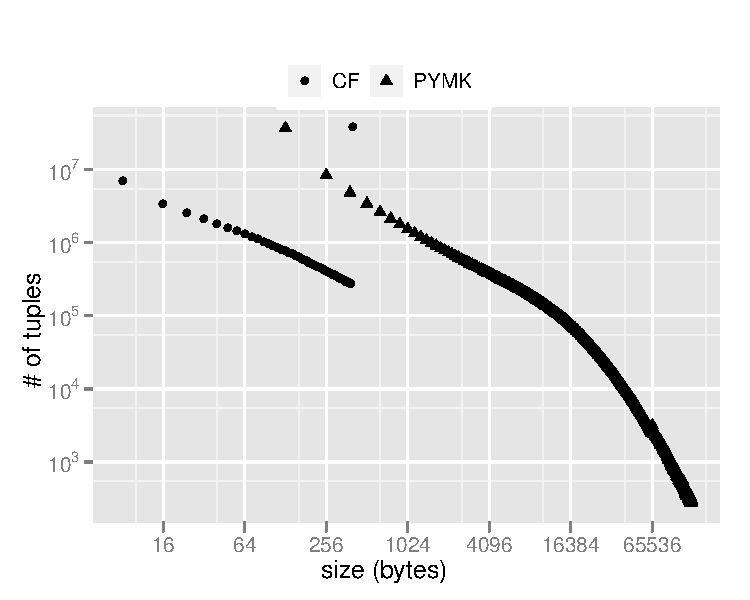
\includegraphics[scale=0.55]{images/data_distribution.pdf}
  \caption{Value size distributions for PYMK and CF. The abrupt stop
is due to the cap on the number of recommendations.}
  \label{distribution}
\end{figure}

\subsection{Build times}

One of the important goals of \projectname{} is rapid data deployment,
which means the build and push phase must be fast. Push times are
entirely dependent on available network bandwidth, so we focus on
build times.
 
To ensure fair comparisons, we built all our stores on a single node.
The build time in case of \projectname's Hadoop workflow includes the
time to generate the chunk mapping in the map phase, shuffle the data,
and finally, in the reduce phase, emit the store files. The number of
mappers and reducer are kept fixed so as to have same amount of
parallelism. This also resulted in fixed number of chunks being
generated.

In case of MySQL, the MyISAM test is the completion time of the
\sql{LOAD DATA INFILE} command. Some optimizations to make MySQL
faster include increasing the MySQL bulk insert buffer size and the
MyISAM specific sort buffer size to 256 MB each and delaying the
re-creation of the index to a latter time by running \sql{ALTER
TABLE...DISABLE KEYS} statement before the load. 

Besides the B$^{+}$ tree structure built inside MySQL, we build our
own B$^{+}$ tree structure tailored to Hadoop. Instead of generating
chunk files in every reducer step, we generate a B$^{+}$ tree. This
tree contains of a single data file, similar to the chunk data file,
and a set of index files corresponding to every level of the tree. The
bulk loading of the tree is done in blocks (of size~$b$); that is, the
system first finishes the lower level's block and only then
initializes a block at the next level. The system applies this rule
recursively for every level as the sorted elements stream through.
This bulk loading approach is efficient in that it does not require
buffering any values in memory and the system can directly write to
the level-based index files. 

Figure~\ref{build} shows the build time as we increased the size of
the input data-set. The block size~$b$ for the B$^{+}$ was set to~340,
which was chosen as the keys were 12~bytes long (8~byte MD5 and 4~byte
offset) and the system page size is~4096 bytes. This meant the best
block size would be approximately $4096/12 \sim 340$. As is clearly
evident, MySQL exhibits extremely slow build times even after being
alloted a huge buffer size. The optimized B$^{+}$, on the other hand,
performs well for small sizes but deviates at larger input sizes due
to the extra I/O required: extra disk writes for the higher levels of
the tree are necessary. For a fixed block size, the extra disk writes
are linear with the number of tuples.  Another disadvantage of the
B$^{+}$ tree approach is that the serving latency is sensitive to the
block size~$b$, which is machine-specific. 

\begin{figure}
  \centering
    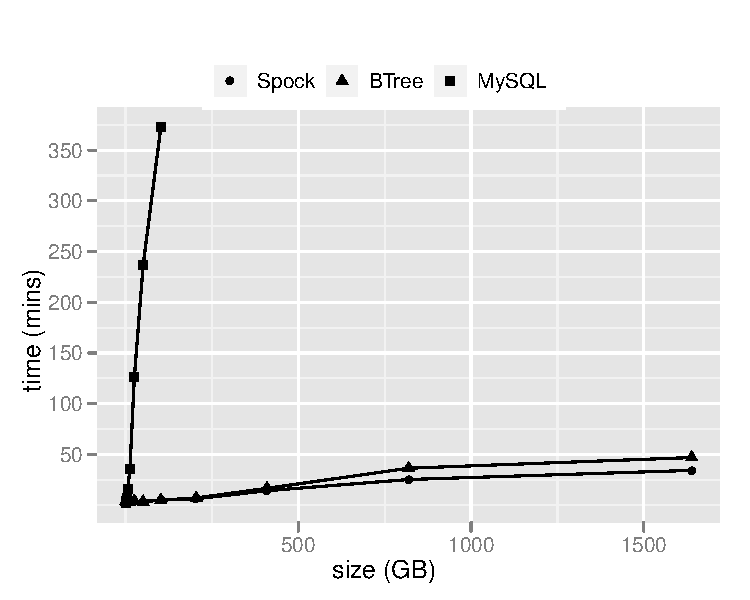
\includegraphics[scale=0.55]{images/build.pdf}
  \caption{Build time vs varying data size}
  \label{build}
\end{figure}

\subsection{Read latency}

Besides rapid data deployments, the read latency must be acceptable
and the system must scale with the number of nodes. For the random
data-set, we used 10~million requests with simulated values following
a uniform distribution. For the PYMK and CF data-set, we use a
snapshot of member activity for one high traffic day.

We first try to understand the performance implications of binary
search against interpolation search. In particular, we are interested
in measuring how fast the index can get paged into the OS's page
cache. We ran tests on a 100~GB of data on a single node with the page
cache being flushed between test runs. Figure~\ref{search} shows the
median latency over time. Binary search initially starts with a high
median latency, but the slope of the line is steeper compared to that
of interpolation search. This is because binary search did an average
of 17.5~lookups thereby touching more parts of the index;
interpolation search, on the other hand, performs only 4~lookups.
While this results in an initial low read latency, it comes at the
expense that much of the index is uncached in the long run. Our
production systems are currently running binary search due to this
faster cache warming process.  

\begin{figure}
  \centering
    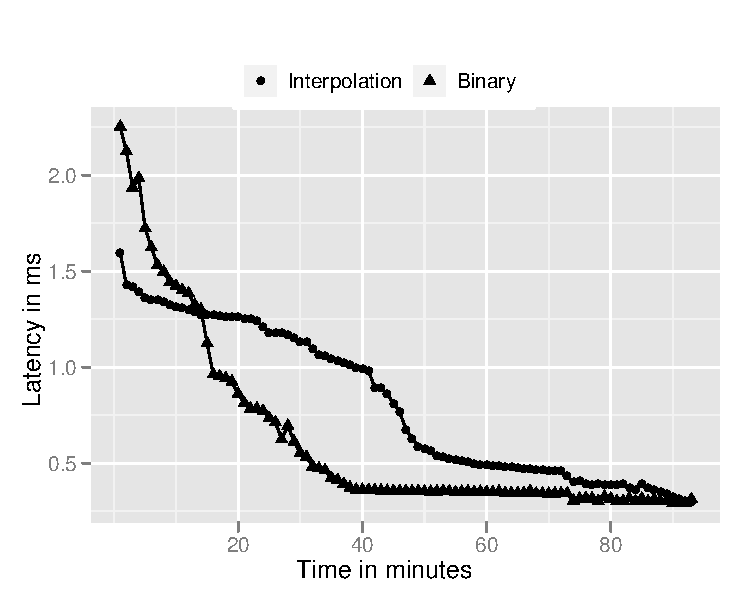
\includegraphics[scale=0.55]{images/search_1node.pdf}
  \caption{Search Latency vs Time since swap}
  \label{search}
\end{figure}

Table~\ref{mysql:search} shows a comparison of \projectname's
performance to MySQL on the same 100~GB data-set for a fixed
throughput of 1000~queries per second. Our optimizations for the
read-only case have resulted in faster serve times: 75% decrease in
median latency with 20% less latency in the 99th quantile. 

\begin{table}
\centering
\begin{tabular}{ | c | c | c |  }
\hline
                & MySQL   & \projectname{} \\ \hline
Median          & 0.12 ms & 0.028 ms       \\
99th quantile	& 45 ms   & 36 ms          \\
\hline
\end{tabular}
\caption{}
\label{mysql:search}
\end{table}

To test whether the system scales well with the number of nodes, we
present read latency numbers for the same random data-set but spread
over 16~machines. The data was fetched by \projectname{} at a steady
rate bound by the network; we saturated the 1~Gbit line between HDFS
and \projectname{} nodes. We ran the tests for both uniform as well as
a Zipfian distribution~\cite{gray}. In particular, we ensure that the
hot elements are queried together since that simulates the general
site visiting patterns of most websites~\cite{...}.
Figure~\ref{16search} shows the maximum median latency of each
individual node with varying data-set sizes. The hotness of a few keys
naturally aids cachability, thereby exhibiting an overall lower
latency compared to the uniform distribution. 

\begin{figure}
  \centering
    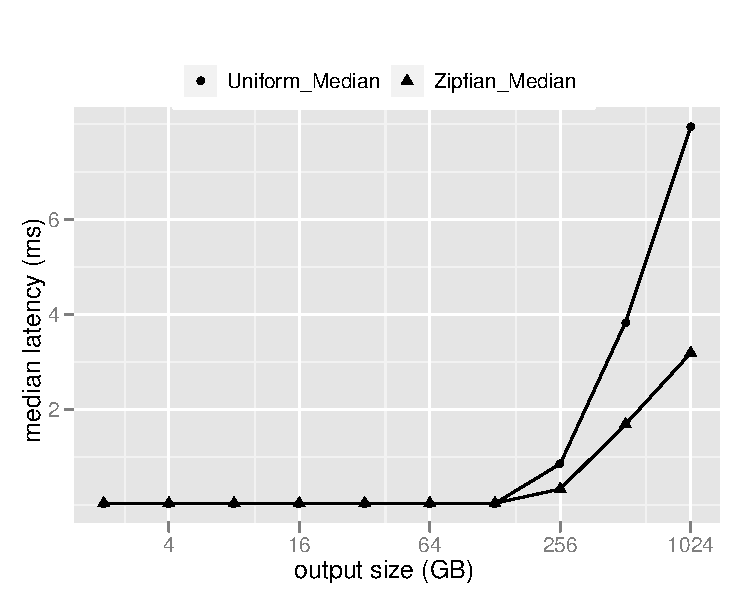
\includegraphics[scale=0.55]{images/search_16node.pdf}
  \caption{Median search latency vs varying data size for 16 node cluster}
  \label{16search}
\end{figure}

Finally, Figure~\ref{production} shows the PYMK and CF read latencies
in our production cluster. The figure shows the average latency across
all server nodes immediately after a new data swap. CF has a higher
latency primarily because of the larger data size than that of PYMK.

\begin{figure*}
  \centering
    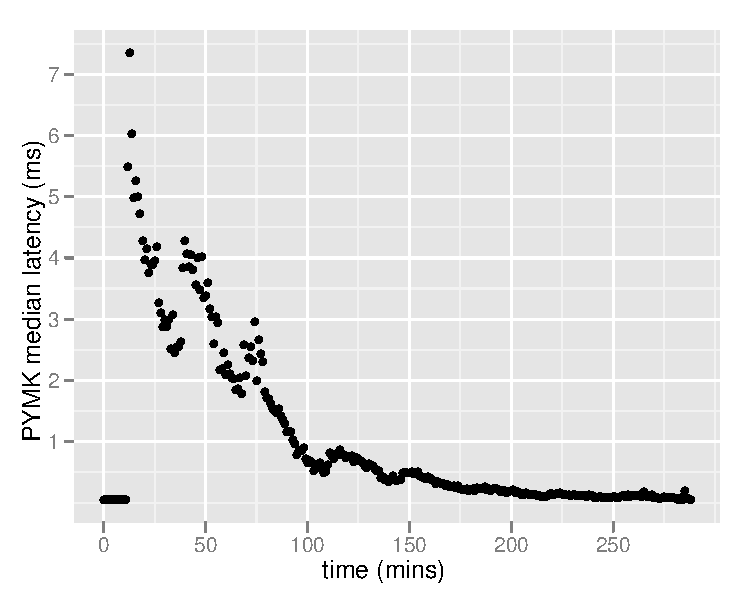
\includegraphics[scale=0.55]{images/pymk_search.pdf}
    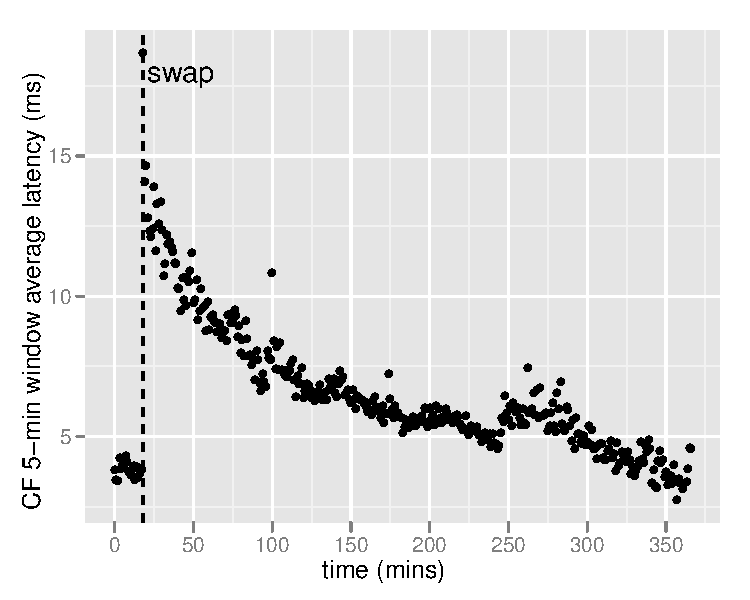
\includegraphics[scale=0.55]{images/browsemap_search.pdf}
  \caption{Latency vs Time for PYMK and CF}
  \label{production}
\end{figure*}

